%%%%%%%%%%%%%%%%%%%%%%%%%%%%%%%%%%%%%%%%%%%%%%%%%%%%%%%%%%%%%%%%%%%%%%%%%%%%%%%%%%%%%%%%%%%%%%%%%%%%%%%%%%%%%%%%%%%%%%%%%%%%%%%%%%%%%%
%Navrhněte nasazení řešení BYOD. 

V této kapitole bude podrobně popsán návrh řešení pro BYOD program ve vybrané organizaci. Volba produktů pro uskutečnění řešení bude odůvodněna a taktéž bude popsána jejich funkcionalita. Závěr kapitoly se věnuje nasazení vybraného řešení jak po technické stránce, tak po stránce formální. 


\section{Návaznost na stávající řešení}
%\todo{napsat}
V Bance existuje projekt pro centralizovanou virtualizaci. Navržené řešení na tento projekt nenavazuje a navrhuje jiný přístup. Zároveň je nasazována infrastruktura pro použití BlackBerry Work. Tato práce na toto řešení navazuje a rozšiřuje jeho použití jako součást koncepce návrhu uceleného BYOD programu. 

Použitá síťová infrastruktura ve firmě je nyní vcelku komplexní. Navržené řešení se snaží nasazené infrastruktury využít a nenavrhuje žádné významné změny. 

Stávající proces připojování nefiremních zařízení by měl být nahrazen zařazením nefiremních zařízení do uceleného BYOD programu


\section{Návrh řešení pro notebooky}

Banka nehledá komplexní řešení pro virtualizaci pracovních stanic. Stávající situace, kdy zaměstnanci používají firemní zařízení je vyhovující a není důvod do ní jakkoli výrazněji zasahovat. Je však třeba najít odpověď na narůstající trend vlastních zařízení a především představit rámec pro kontraktory, kteří firemním zařízení nedisponují tak, aby nebyli rizikem pro vnitřní síť a jejich chování v rámci sítě bylo kontrolováno firemními politikami.

%\todo{Návaznost na kapitolu kde analizuju KB BYOD podle prezentace}

Vzhledem k nárokům kladeným na BYOD v Bance, viz \ref{obecnePozadavky}, vychází jako řešení nejlépe distribuovaná virtualizace. Navržené řešení umožňuje pokročilou správu distribuovaných virtuálních strojů nutnou pro plnění firemních politik, odděluje pracovní prostředí od soukromého operačního systému, viz \ref{analyzaRizik}, neklade vysoké náklady na konektivitu a síťovou infrastrukturu, viz \ref{projektVDI}, a dokonce umožňuje práci offline. Jediným uceleným řešením s distribuovanou virtualizací a současnou možností vzdálené správy klientů je  VMware Horizon FLEX. Tato práce jako řešení BYOD pro notebooky tedy navrhuje produkt VMware Horizon FLEX.



\subsection{VMware Horizon Flex}
V roce 2014 VMware představil VMware řešení VMware Horizon Flex. Jedná se o kombinaci některých stávajících technologií jako je Fusion, Player, Mirage či AirWatch. Dle \cite{GartnerFlex} je odpovědí na požadavky zákazníku provozovat virtuální desktopy offline. Zároveň přináší výhody virtualizace, ale nenese s sebou velké náklady v podobě nutnosti výkonných serverů a dostatečného diskového úložiště jako v případě centralizované virtualizace, což byl jeden s hlavních důvodů, proč centralizovaná virtualizace ve zkoumané organizaci není rozšířena jako alternativa pro řešení BYOD, viz (\ref{projektVDI}). Nevýhoda virtualizace v podobě vysokých nároků na konektivitu a špatné odezvy je u tohoto řešení taktéž neexistující. 

Uživatelé mohou přistupovat do korporátní sítě z korporátního obrazu operačního systému, ale přitom používat své vlastní notebooky nebo počítače od firmy Apple, bez toho, aby tyto zařízení muselo IT oddělení podporovat. IT může plně spravovat korporátní systém bez toho, aby zasahovalo do operačního systému uživatele. Bezpečnostní rizika jsou minimalizována díky oddělení obou operačních systémů a možnosti vzdáleně řídit omezení pro virtuální stoj, či ho dokonce vzdáleně uzamknout či smazat. Tato možnost je obzvláště výhodná u externích pracovníků, kterým může vypršet kontrakt. Do systému Horizon FLEX je možné zapojit také obrazy virtuálních strojů sloužící pro testování a lépe je tak spravovat.

Technicky se jedná o hypervizor typu 2, který je spravovaný centrálně. Je možné jej nasadit jak pro koncové stanice s Mac OS, tak s Windows. Spravovat, zálohovat a záplatovat systém je též možné centrálně, a to s užitím serveru Mirage for Horizon FLEX. Pro nastavení politik řešení obsahuje Horizon FLEX Policy Server, jako klient je použit VMware Fusion Pro pro počítače Mac a VMware Workstation Player pro počítače s Windows, viz \cite{FlexBrief}. % \todo{citovat %http://www.vmware.com/content/dam/digitalmarketing/vmware/en/pdf/techpaper/ vmware-horizon-flex-solution-brief-mirage-fusion-player.pdf}
Pro klienta jsou podporovány následující 64bitové operační systémy: Windows 7, Windows 8.1, Windows 10, Mac OS X 10.9, Mac OS X 10.10 a Mac OS X 10.11.

 \begin{figure}[h!]
 \centering
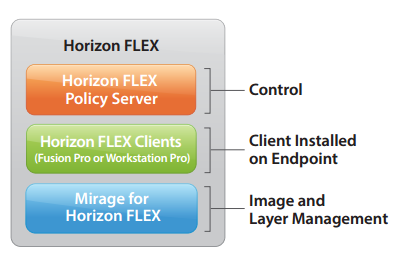
\includegraphics[width=8cm]{img/FlexVrstvy}
\caption{Vrstvy produktu VMWare Horizon FLEX. Převzato z: \cite{FlexBrief}} 
\label{FlexVrstvy}
\end{figure}%\todo{citovat %http://www.vmware.com/content /dam/digitalmarketing/vmware/ en/pdf/techpaper/ vmware-horizon-flex-solution-brief-mirage-fusion-player.pdf}



Různě nastavené virtuální stroje je možné distribuovat různým uživatelům. Uživateli musí být nejdříve nainstalován klient a tedy Fusion Pro nebo Workstation Player. Uživatelský systém potřebuje přístup k Horizon FLEX Policy serveru v následujících případech: pro úvodní stažení obrazu stroje a pro získání aktualizací politik a omezení. Horizon Flex Policy Server musí být pro klienta dostupný pomocí protokolu https. Je možné nastavit maximální počet dní bez připojení k Policy Serveru. Minimimální hardwarové požadavky serverů jsou sepsány v příloze (\ref{pozadavky})


 \begin{figure}[h!]\label{FlexPolicy}
 \centering
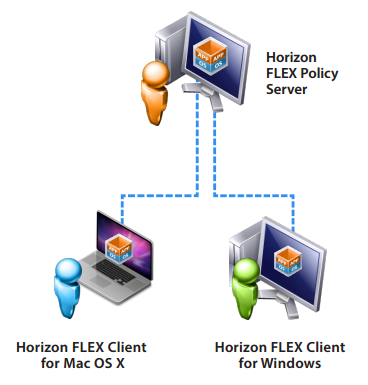
\includegraphics[width=6cm]{img/FlexPolicy}
\caption{Schéma pro připojení k Horizon Flex Policy serveru. Převzato z: \cite{FlexBrief}}
\end{figure}%\todo{citovat %http://www.vmware.com/ content/dam/digitalmarketing/ vmware/en/pdf/techpaper/ vmware-horizon-flex-solution-brief-mirage-fusion-player.pdf} 


S užitím Policy serveru mohou administrátoři mimo jiné spravovat inventář omezených virtuálních strojů, procházet seznam uživatelů a skupin ve službě Active Directory, přiřazovat uživatele a skupiny k jednomu či více virtuálnímu stroji, specifikovat politiky pro dané přiřazení, omezit uživateli přístup k virtuálnímu stroji vzdáleným zamknutím nebo kontrolovat stav virtuálního stroje.

Pro nastavování politik slouží webové uživatelské rozhraní. Je možné nastavit následující omezení:

\begin{itemize}
    \item Expirační doba -- Doba, po kterou je virtuální stroj přístupný.
    \item Použití USB zařízení -- Blokování použití zvolených USB zařízení.
    \item Copy\&Paste operace -- Omezení funkce copy and paste mezi hostitelským a virtualizovaným operačním systémem.
    \item Drag\&Drop operace -- Omezení drag and drop funkcionality mezi hostitelským a virtualizovaným operačním systémem.
    \item Zadaní hesla pro kopírování či přesouvání virtuálního stroje.
    \item Omezení existujících instancí virtuálního stroje na jednu.
    \item Omezení možnosti přidělování hardwarových prostředků pro virtuální stroj.
\end{itemize}

Virtuální stroj je též možné vzdáleně uzamknout a nebo smazat.

\subsection{Doporučení pro korporátní obraz virtuálního stroje}
Obraz virtuálního stroje by měl odpovídat nastavení operačního systému pro firemní zařízení. Speciálním omezením by mělo být vynucení přístupu do sítě pouze prostřednictvím firemní VPN.

\subsection{Dodatek návrhu pro uživatele s operačními systémy linuxového typu}
Řešení Horizon Flex bohužel nepodporuje operační systém Linux. Pro tento specifický typ uživatelů je tedy třeba navrhnout alternativu. Jelikož klient řešení Horizon Flex je produkt VMware workstation Pro, je vhodné pro zachování konzistence návrhu uživatelům operačního systému Linux navrhnout tohoto klienta. VMware Workstation for Linux podporuje následující operační systémy: Ubuntu 8.04 a vyšší, Red Hat Enterprise Linux 5 a vyšší, CentOS 5.0 a vyšší, Oracle Linux 5.0 a vyšší, open SUSE 10.2 a vyšší, SUSE Linux 10 a vyšší. U dalších distribucí systému typu Linux a Unix není oficiální podpora, ale řešení může být funkční.

V tomto klientu je možné spouštět zašifrované omezené virtuální stroje určené pro Horizon Flex. Vzhledem k neexistenci komunikace s Policy serverem však není možné nastavené politiky dodatečně měnit či vzdáleně smazat či spravovat obraz virtuálního stroje. Přístup do stroje a firemní sítě je však možné znemožnit zneplatněním přístupu daného uživatele skrze Active directory a tedy jedná se stále o bezpečné řešení.

\subsection{Licencování}
Licence na Horizon Flex se vztahuje k zařízení. Prodávají se pouze v balících. Jeden balík obsahuje 10 licencí pro klienta a licenci pro VMWare Mirage For Flex a Horizon FLEX Policy Server.

Pro klienty VMware Workstation For Linux je třeba zakoupit zvláštní licenci.


\section{Návrh řešení pro mobilní zařízení}

Z analýzy požadavků uživatelů, viz \ref{identifikovaneSluyby}, vyplynulo, že pro mobilní telefony je požadována především dostupnost emailu a pro tablety je to především dostupnost emailu, dokumentů a PIM. Z hlediska požadavků byznysu je to vzhledem k povaze bankovního sektoru především vysoká bezpečnost.

Přestože leaderem trhu EMM je řešení AirWatch od společnosti VMware, v klíčových vlastnostech není nejsilnější. AirWatch je vysoce modulární řešení schopné plnit vysoké nároky. Jeho slabou stránkou je PIM, kde je doporučeno použít řešení od třetí strany.

V klíčových požadavcích exceluje řešení od společnosti BlackBerry. Pro email a PIM nabízí kvalitní produkt BlackBerry Work. V oblasti bezpečnosti je společností Gartner hodnocen, viz \cite{GartnerSecurity}, jako nejsilnější hráč na trhu. %\todo{citace %https://www.gartner.com/ doc/reprints?id=1-3GSO3TQ \&ct=160902\&st=sb}.
Tato práce navrhuje jako řešení BYOD pro mobilní telefony a tablety řešení BlackBerry Enterprise Mobility Suite.

\begin{figure}[h!]\label{GartnerBB}
\centering
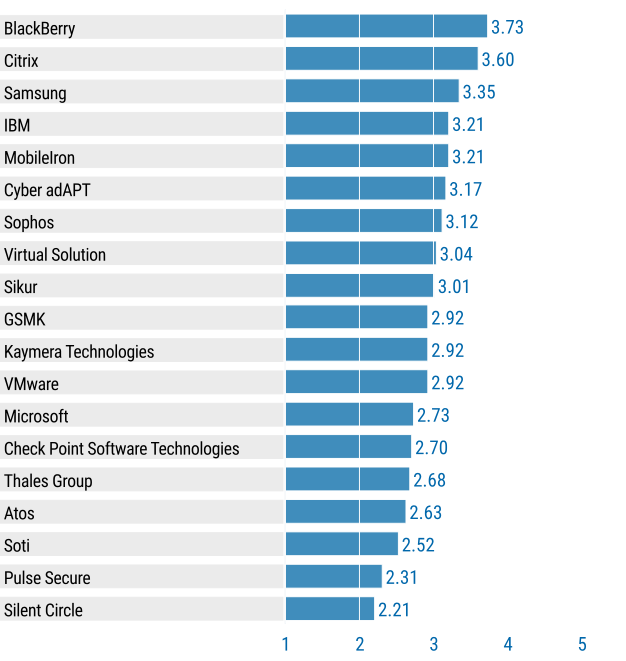
\includegraphics[width=10cm]{img/GartnerBB}
\caption{Hodnocení dodavatelů software pro vysoce bezpečnou správu mobilních zařízení v kategorii BYO od společnosti Gartner. Převzato z: \cite{GartnerSecurity}}
\end{figure}%\todo{citovat %https://www.gartner.com/doc/ reprints? id=1-3GSO3TQ\&ct=160902\&st=sb} 

Společnost Gartner hodnotila produkt v několika kategoriích. 

Z hlediska certifikací a ocenění je situace rozdílná pro každou aplikaci v balíku. Good Dynamics je certifikován jako EAL4+. Kryptografické komponenty jsou certifikovány jako FIPS 140-2 Level 1. Mezi další certifikace, které splňují komponenty od Good technologies patří například ISO 19790 či další státní a armádní normy.

Co se týče MDM, nabízí BlackBerry všechny běžné funkce. Platforma podporuje Android for Work i Samsung Knox. Kontejnerizaci aplikací zajišťuje komponenta Good Dynamics. Je možné chránit aplikace hesly a přiřazovat jim certifikáty. Kontejnery mezi sebou mohou komunikovat s užitím certifikátů podepsaných backendovým serverem. 


Dalším důvodem pro volbu BlackBerry je použití tohoto řešení v mateřské firmě. Během analýzy bylo zjištěno, že toto řešení se připravuje také pro KB, a že během vypracovávání této diplomové práce začala fáze plošného nasazování. Jelikož je řešení od BlackBerry podle analýzy požadavků v této práci nejvhodnějším řešením, tato práce nasazení zvoleného řešení podporuje. Řešení je integrovatelné s řešením od různých poskytovatelů NAC včetně použitého řešení od Cisca.    


\section{BlackBerry Enterprise Mobility Suite}

Nejdůležitější komponentou pro potřeby Banky je BlackBerry Work. Dle specifikací \cite{BBSpecs}%\todo{citovat %https://ca.blackberry.com/ enterprise/gfe-comparison}
 nabízí následující funkcionalitu:

Email:
\begin{itemize}
    \item Synchronizace emailu
    \item Správa emailu
    \item Zabezpečené zobrazování příloh
    \item Správa fotografií
    \item Vyhledávání emailů na serveru
    \item Prioritizace oznámení
    \item Inegrace s nositelnostmi
\end{itemize}

Kalendář:
\begin{itemize}
 \item Synchronizace kalendáře
 \item Připojení ke konferenčním hovorům
 \item Plánování meetingů
 \item Zprávy "mimo kancelář"
 \item Zobrazení přijatých pozvánek
\end{itemize}

Kontakty:
\begin{itemize}
   \item Synchronizace kontaktů
   \item Vyhledávání v pracovních kontaktech přímo z telefonu
   \item Historie zpráv
\end{itemize}

Kolaborace:
\begin{itemize}
   \item Ukládání souborů do repozitáře
   \item Zabezpečený prohlížeč pro přístup k firemnímu intranetu
   \item Správa úkolů
   \item Přístup k dokumentům ve službách SharePoint, OneDrive nebo Box
   \item Prezentační mód pro prezentaci PowerPoint dokumentů
\end{itemize}

Zajímavou funkcí je jednoduchý přístup pomocí funkce Touch ID na zařízeních s operačním systémem iOS podporující funkci Touch ID.\\

Možnoti administrace:
\begin{itemize}
   \item Šifrovaný kontejner
   \item Integrované MDM
   \item Jednotný dokumentový server
   \item Integrované MAM
   \item Použití technologie Exchange ActiveSync
   \item Rozdělení účtování dat na pracovní a soukromý provoz
\end{itemize}

\subsection{Návrh licencování}

Nejnutnější funkce pro splnění požadavků předpokládaných uživatelů BYOD splňuje komponenta BlackBerry Work. Ta je součástí skupiny služeb BlackBerry Dynamics. Aplikace BlackBerry Dynamics se licencují pouze jako součást balíku Blackberry Enterprise Mobility Suites, který je nabízen v různých edicích.

Pro splnění požadavků na funkce emailu postačuje edice BlackBerry Enterprise Mobility Suite --  Enterprise Edition. Pro pokročilejší práci s dokumenty vyžadovanou pro BYOD tablety je třeba zakoupit vyšší edici BlackBerry Enterprise Mobility Suite -- Collaboration Edition, viz \cite{BBEMS}.% \todo{ citovat datasheet %https://global.blackberry.com/ content/dam/blackberry-com/PDF/enterprise/ ds-blackberry-enterprise-mobility-suite.pdf}.
 Tato vyšší edice je též třeba pro integraci s IM klientem Skype for Bussiness.

Tato edice nabízí následující typy aktivace: Work and personal - Regulated, Work space only, Work and personal - user privacy (Android for Work -- Premium), Work space only (Android for Work - Premium), Work and personal - user privacy (Samsung KNOX), Work and personal - full control (Samsung KNOX), Work space only (Samsung KNOX). Nabízí tedy vhodné možnosti jak pro BYOD zařízení, tak pro správu firemních zařízení. 

Pro BYOD mobilní telefony s operačním systémem Android je tedy vhodná licence BlackBerry Enterprise Mobility Suite -- Enterprise Edition a typ aktivace Work and personal -- user privacy.

Pro BYOD mobilní telefony s operačním systémem iOS je vhodná licence BlackBerry Enterprise Mobility Suite -- Enterpirse Edition a typ aktivace user privacy.

Pro BYOD tablety s operařním systémem Android je nejvhodnější licence BlackBerry Enterprise Mobility Suite -- Collaboration Edition a typ aktivace Work and personal - user privacy (Android for Work - Premium).

Pro BYOD tablety s operačním systémem iOS je nejvhodnější licence BlackBerry Enterprise Mobility Suite -- Collaboration Edition a typ aktivace User privacy.

Pro všechny BYOD užití je vhodnější serverový typ licence.

Informace o licencování byly čerpány z oficiální dokumentace \cite{BBLicence}.% \todo{citovace %http://help.blackberry.com/ en/blackberry-uem/12.6/licensing/ dhd1465315353877.html}.

%%%%%%%%%%%%%%%%%%%%%%%%%%%%%%%%%%%%%%%%%%%%%%%%%%%%%%%%%%%%%%%%%%%%%%%%%%%%%%%%%%%%%%%%%%%%%%%%%%%%%%%%%%%%%%%%%%%%%%%%%%%%%%%%%%%%%
%Konzultujte navrhované řešení se zástupci vybrané organizace a stanovte doporučení pro nasazení. 
\section{Hodnocení navrhované varianty zástupci organizace}
Zástupci vybrané společnosti ohodnotili návrh jako jako splňující požadavky. Ocenili především splnění nároků na bezpečnost díky důslednému oddělení soukromého a pracovního prostředí. Z hlediska nasazení je hodnocen jako proveditelný, přičemž detailní plán nasazení by musel být analyzován a schválen dalšími odděleními vzhledem k zásahům do infrastruktury a součinnosti s jinými běžícími projekty. 
Úskalím projektu by mohlo být vyjednávání o zapojení do programu s externími dodavateli a kontraktory.

\section{Návrh nasazení řešení pro notebooky}
\todo{citovat %http://www.vmware.com/content/dam/digitalmarketing/vmware/en/pdf/techpaper/vmware-horizon-flex-deployment-considerations.pdf
}

V první řadě je třeba vyhradit prostor na kterém budou umístěny obrazy pro virtuální stroje. Je vhodné připravit souborové servery pomocí IIS a to jeden uvnitř podnikové sítě a jeden vně. Dále je potřeba nainstalovat Mirage Management server a jeho komponenty. Při zadání sériového čísla se zpřístupní funkce pro Horizon FLEX, viz \cite{FlexDeployment}. 

Jelikož se v prostředí Banky používá operační systém Windows, pro vytvoření obrazu pro virtuální stroj je potřeba použít nástroj VMware Workstation Pro, viz. obrázek \ref{workstation}

\begin{figure}[h!]
\centering
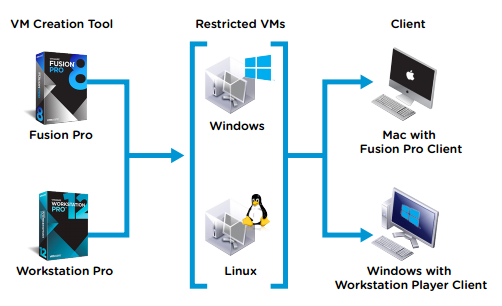
\includegraphics[width=10cm]{img/workstation}
\caption{Schéma postupu pro vytvoření obrazu virtuálního stroje. Převzato z: \cite{FlexDeployment}}
\label{workstation}
\end{figure}%\todo{citovat %http://www.vmware.com/content/ dam/digitalmarketing/vmware/en/ pdf/techpaper/vmware-horizon-flex-deployment-considerations.pdf} 




\begin{figure}[h!]
\centering
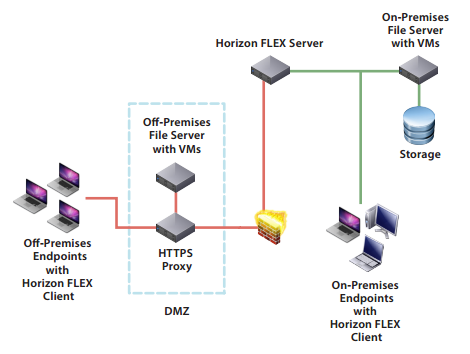
\includegraphics[width=10cm]{img/schemaArchitektury}
\caption{Ilustrační schéma infrastruktury pro nasazení VMware Horizon FLEX. Převzato z: \cite{FlexDeployment}}\label{schemaArchitektury}
\end{figure}%\todo{citovat %http://www.vmware.com/content/ dam/digitalmarketing/vmware/en/pdf/techpaper/vmware-horizon-flex-deployment-considerations.pdf} 


Po instalaci serveru Mirage je třeba nainstalovat nainstalovat ostatní komponenty Horizon FLEX, nastavit certifikáty pro virtuální stroje, vytvořit a přiřadit virtuální stroje a nakonec nainstalovat klienty na koncová zařízení. Klienty je možné distribuovat uživatelům s připravenými virtuálními stroji. 

Jelikož jeden Horizon FLEX Server dokáže obsloužit až 10000 uživatelů, stačil by pro potřeby organizace pouze jeden server. Firemním standardem je však zajistit u podobných služeb vysokou dostupnost.




\section{Návrh nasazení řešení pro mobilní zařízení}
Jelikož nasazení řešení v Komerční bance již započalo, návrh nasazení soustředí spíše na popis a využitelnost řešení, než-li na technickou specifikaci návrhu pro nasazení.

\subsection{Komponenty řešení}


Základním kamenem řešení je BlackBerry Unified Endpoint Management (UEM). %\todo{cituju %http://help.blackberry.com/en/blackberry-uem/current/}
Jedná se o infrastrukturu pro zajištění MDM, viz \cite{BBUEM}. BlackBerry Infrastructure je vnější server, který spravuje informace o zařízení jako jsou licence a šifrovaně komunikuje s UEM a také s koncovými zařízeními.

\begin{figure}[h!]\label{BBUEM1}
\centering
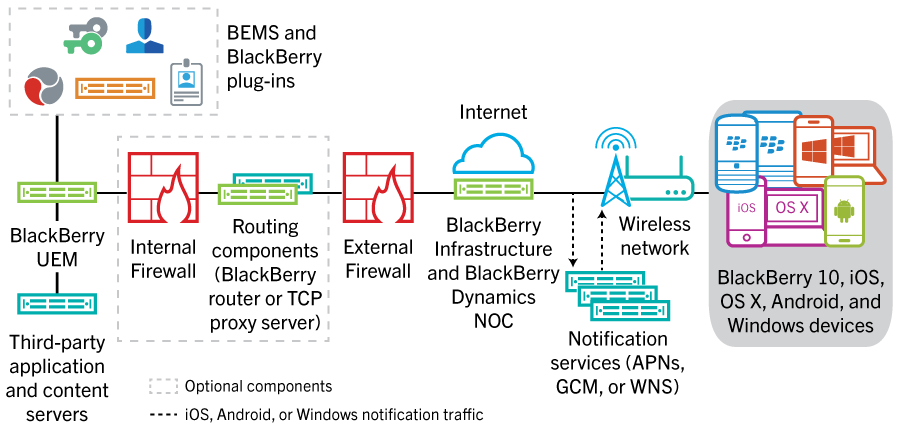
\includegraphics[width=12cm]{img/BBUEM1}
\caption{Architektura BlackBerry UEM. Převzato z \cite{BBUEM}.}
\end{figure}%\todo{citovat %http://help.blackberry.com/ en/blackberry-uem/current/} 

Pro potřeby splnění požadavků na BYOD je potřeba nasadit další komponenty balíku BlackBerry Enterprise Mobile Suite na úrovni edice Collaboration Edition. Na obrázku \ref{BBEMS} jsou jednotlivé komponenty rozkreslené.

\begin{figure}[h!]
\centering
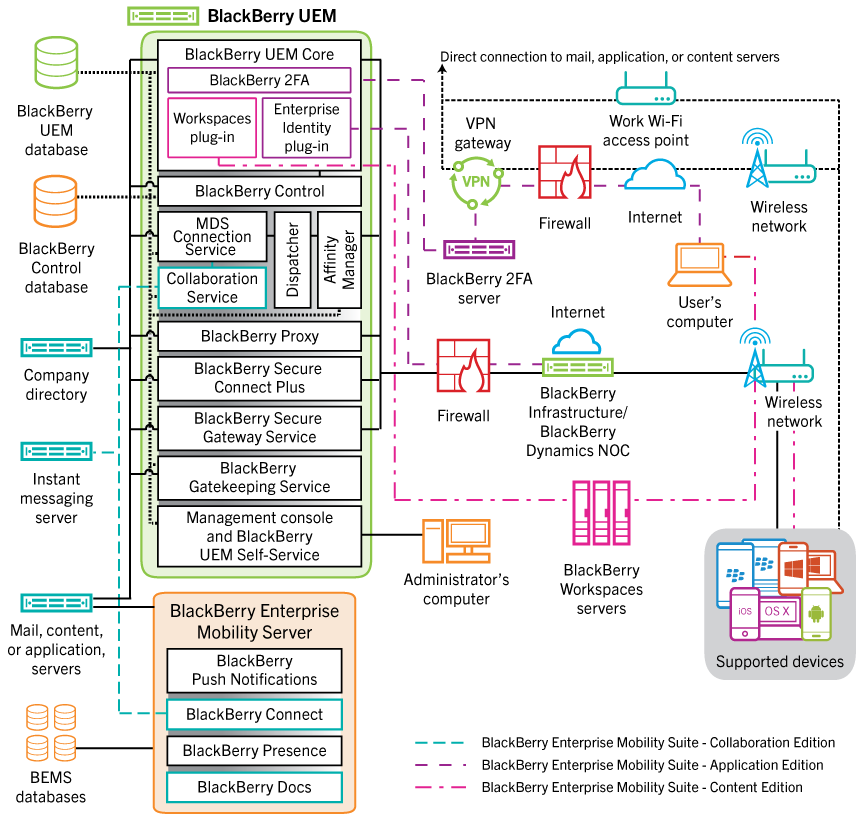
\includegraphics[width=13cm]{img/BBEMS}
\caption{Schéma komponentů balíku BlackBerry Enterprise Mobility Suite. Převzato z: \cite{BBUEM}}\label{BBEMS}
\end{figure}%\todo{citovat %http://help.blackberry.com/ en/blackberry-enterprise-products/ latest/enterprise-products/ eqg1459529064051.html} 

Jádrem řešení je BlackBerry UEM, který dále obsahuje subkomponenty jako jsou mimo jiné logování, monitoring, reportování, funkce pro správu, služby pro autentifikaci a autorizaci, plánování a zasílání příkazů či IT politiky a profily zařízení. BlackBerry Control slouží k zasílání konfiguračních dat do aplikací BlackBerry Dynamics v koncových zařízeních. BlackBerry Collaboration Service poslouží k propojení se službou Microsoft Skype For Business. 

BlackBerry Enterprise Mobility Server slouží k posílání dat do BlackBerry Dynamics Apps. Většina funkcí je využitelná až u vyšších edicí BlackBerry Enterprise Mobility suite.

\subsection{Kroky instalace}
V první řadě je třeba nainstalovat BlackBerry UEM. Dále je třeba nainstalovat BlackBerry Enterprise Mobility Server. V rámci tohoto severu je třeba nakonfigurovat BlackBerry Dynamics a nastavit certifikáty.  Dále je třeba nastavit přístup do Active directory, SMTP server a Exchange ActiveSync. Dalším krokem je nastavení konektivity pro BlackBerry Dynamics. Po té je nutné nastavit BlackBerry Dynamics profil a zpřístupnit tak uživatelům aplikace BlackBerry Work a BlackBerry Access. 

V BlackBerry dynamics je možné nastavit některé politiky. Pro účely BYOD zařízení je třeba nastavit zamezení přístupu uživatelům s operačním systémem umožnující administrátorské operace (JailBreak/Root) a nastavit interval nutný pro synchronizaci s UEM.

Posledním krokem je nastavení uživatelských účtů a skupin. Aktivace z hlediska uživatele spočívá v instalaci software BlackBerry UEM a BlackBerry Work z obchodu s aplikacemi pro svůj operační systém. Další postup aktivace je triviální.

Maximální počet uživatelů na jeden server 20 000, což znamená, že KB bude stačit jediný server. 

\subsection{Integrace s Cisco ISE}

BlackBerry UEM je možné integrovat s Cisco ISE, čož je NAC prvek používaný v Bance. Díky této integraci ISE může od UEM získávat data o zařízení, na základě kterých může povolit nebo zamítnout přístup zařízení do firemní sítě, viz \cite{CiscoDesign}.

Cisco ISE vyžaduje v UEM vlastní administrátorský profil, ten je třeba nastavit. Dále je třeba importovat do ISE BlackBerry Web Service Certificate exportovaný z UEM. V ISE je nyní možné nastavit připojení k UEM. 

Nyní může ISE získávat data o zařízení jako je MAC adresa, splnění politik, nastavení šifrování, informace o aktivaci v UEM, detekce jailbreak, výrobce, model, sériové číslo, verze operačního systému nebo nastavení zaheslování.

Dále je díky integraci přímo z ISE možné vymazat ze zařízení pracovní data nebo jej uzamknout.

\begin{figure}[h!]
\centering
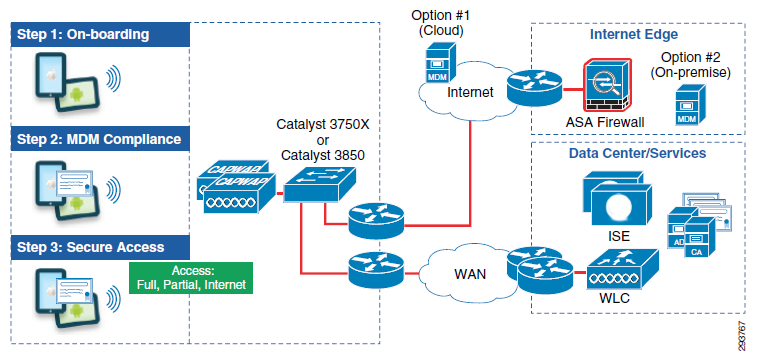
\includegraphics[width=13cm]{img/CiscoMDM}
\caption{Ilustrace připojování uživatelů do sítě s využitím MDM. Převzato z: \cite{CiscoDesign}\label{CiscoMDM}}
\end{figure}%\todo{citovat Cisco design guide} 

Obrázek \ref{CiscoMDM} ilustruje návrh připojování uživatelů k bezdrátové síti s využítím integrace s MDM. Nejdříve se uživatel připojí k SSID pro přihlášení. Po úspěšném přihlášení se uživatel připojí k zabezpečené zaměstnanecké síti. ISE zavolá API MDM serveru, a pokud není registrováno je přesměrováno. V tomto kroku je možné přesměrovat uživatele na stránku produktu BlackBerry UEM obchodu s aplikacemi jeho operačního systému a automatizovat tak jeden z kroků pro nasazení na straně uživatele. Dále ISE získá informace od MDM serveru a do uloží jej do cache. Poté zkontroluje splnění politik. Pokud je kontrola úspěšná, zařízení jsou přiřazena patřičná práva v rámci sítě. Celý postup je vyobrazen v diagramu \ref{CiscoFlow}.


\begin{figure}[h!]
\centering
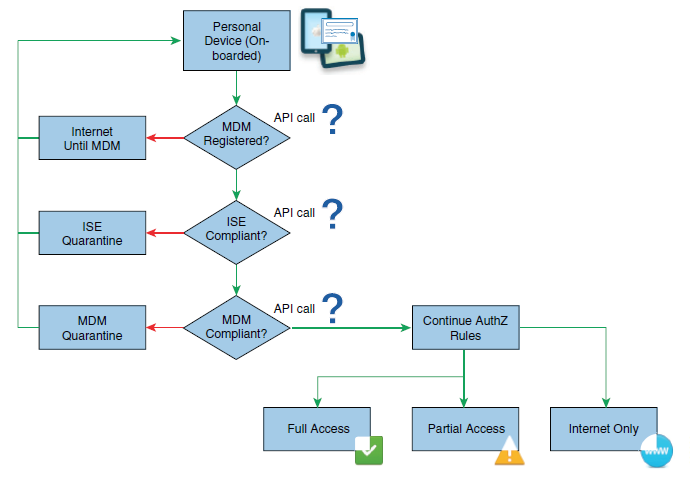
\includegraphics[width=13cm]{img/CiscoFlow}
\caption{Diagram pro připojování zařízení do sítě. Převzato z: \cite{CiscoDesign}.\label{CiscoFlow}}
\end{figure}%\todo{citovat Cisco design guide} 


\section{Síťová infrastruktura nutná k nasazení navrženého řešení pro notebooky}
Navržené řešení neklade zvýšené nároky na síťovou infrastrukturu. Jelikož se jedná o distribuovanou virtualizaci, není třeba zajistit vyšší kvalitu sítě než je běžné.

Pokud by však bylo přistoupeno k oddělení sítě pomocí SSL tunelů, pak by muselo dojít k navýšení kapacity sítě a případně nákupu dalšího nezbytného hardware jako jsou VPN koncentrátory, firewally, routery a podobně -- ne však nezbytně.

Vzhledem k povaze BYOD notebooků se jeví jako nejlepší řešení připojení k internetu pomocí bezdrátové sítě podobného charakteru jaká je k dispozici pro hosty. Přístup do podnikové sítě pak bude zajištěn pomocí VPN. Každý obraz virtuálního stroje bude obsahovat VPN klienta Cisco AnyConnect pro kterého již KB vlastní licence.

Cisco doporučuje \cite{CiscoDesign} odlišit tuto síť od sítě pro hosty několika vylepšeními. Je vhodné umožnit zaměstnancům zajistit si svépomocí přihlašovací údaje a rozšířit možnosti autentifikace o využití Microsoft Active Directory. Taktéž je vhodné narozdíl od síťě pro hosty zajistit vyšší kvalitu služby.

Pro přihlášení k síti se využívá Cisco ISE Sponsor Portal. Po přihlášení je možné porovnat přihlašovací údaje s Active Directory. Taktéž je možné nastavit které skupiny uživatelů mohou udělovat přístupy a monitorovat kdo a kdy přístupy vytvořil. Je vhodné pro BYOD notebooky vytvořit vlastní zabezpečenou síť, viz obrázek \ref{CiscoCUWN}

\begin{figure}[h!]
\centering
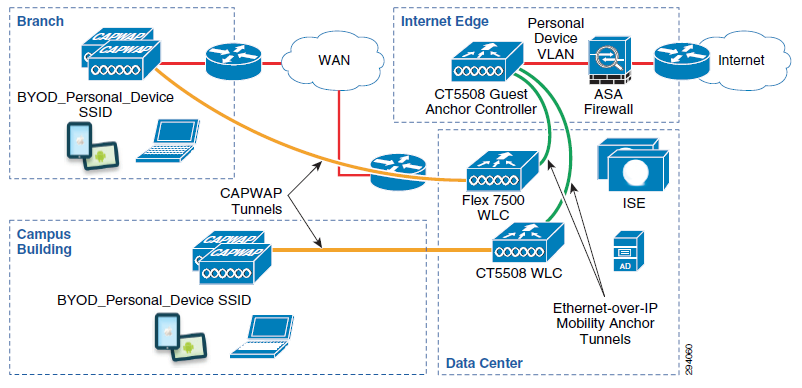
\includegraphics[width=13cm]{img/CiscoCUWN}
\caption{Návrh SSID pro BYOD s využitím technologie Cisco Unified Wireless Network. Převzato z \cite{CiscoDesign}}\label{CiscoCUWN}
\end{figure}%\todo{citovat Cisco design guide} 

Oddělení IT Security však doporučuje nepoužívat bezdrátové sítě a využít stávající kabelovou síť a stávající proces připojování uživatelů s pomocí aplikace MAB Keeper. VLAN přidělená pro BYOD zařízení by poskytovala pouze připojení k internetu a skrze toto připojení by bylo s užitím VPN tunelováno připojení do vnitřní sítě. 



\section{Návrh dalších opatření}\label{dalsi_opatreni}
Další opatření jsou navžena dle sekce \ref{deloitte_aspekty}.

Z hlediska způsobilosti zaměstnanců je navrženu hodnotit způsobilost zaměstnanců pro vstup do BYOD programu. Způsobilost zaměstnance by měl zhodnotit jeho nadřízený. Je nutné určit pro jaké případy jsou vlastní zařízení přípustná a pro jaké nikoliv. Pro zvýšení účinku programu je třeba vynutit vstup do BYOD programu všech, kteří již nyní svá vlastní zařízení k práci používají.

Zaměstnancům využívajícím vlastní zařízení jako náhradu firemního zařízení je nutné vyplácet paušál jako náhradu a toto ošetřit v dodatku pracovní smlouvy. Toto neplatí pro kontraktory.


Není možné podporovat každé BYOD zařízení. Proto se koncept podpory musí změnit na podporu služby. Je třeba zavést uživatelské fórum, na které budou odkázání uživatelé, kteří mají problémy se svými zařízeními, které spadají mimo rámec podpory služby. Je vhodné mít připraveno několik firemních zařízení k zapůjčení připravených jako náhradu pro účastníky BYOD programu s potíži, avšak nezaručovat poskytnutí této služby.

Je třeba vyčlenit pracovníka IT oddělení zodpovědného za BYOD. Ten by měl spravovat návod s postupem pro začlenění zájemců do BYOD programu. Podrobnější školení není nutné.


Je třeba zavést interní směrnici, která ošetří BYOD ve firmě. Je nutné zamezit využívání soukromých zařízení k soukromým účelům v pracovní době. Po náběhu BYOD programu je možné umožnit interními předpisy vstup do BYOD nejenom kontraktorům, ale také vlastním zaměstnancům. Momentálně je toto možné pouze na základě bezpečnostní výjimky. Vstup do BYOD programu ze strany zaměstnanců by měl být dobrovolný. 

Při najímání kontraktorů je třeba brát v úvahu využití konceptu distribuované virtualizace v BYOD programu a tedy smluvně zaručit možnost provozování virtuálního stroje na pracovním zařízení najímaného pracovníka.

Proces pro schvalování bezpečnostních výjimek je třeba zachovat z důvodu neočekávaných mezních případů. Využívání výjimek by však nemělo být možné pro případy užití, které se dají řešit pomocí zapojení do BYOD programu. Zároveň je třeba zachovat smlouvu o užívání vlastního zařízení a aktualizovat ji pro potřeby BYOD programu. Bezpečnostní dotazník a zaručení nadřízeného je díky navrženému BYOD programu z procesu připojování uživatelů s nefiremními zařízeními možné vypustit.

\section{Návrh harmonogramu nasazení}
Jelikož plánování projektů ve vybrané společnosti na rok 2018 je již uzavřeno, bylo by možné projekt pro nasazení BYOD programu naplánovat nejdříve na rok 2019. Pro projekt by bylo třeba najít implementačního partnera, jelikož Banka pro podobné projekty nemá vlastní volné kapacity.

První fází by byla analýza navrženého řešení napříč různými odděleními. Cílem první fáze by bylo určit konkrétní rozsah potřebných změn pro nasazení programu. Výstupem první fáze by byl koncept s jasnými požadavky na konkrétní hardware a organizační změny. Projekt je třeba obhájit před vedením společnosti, a je potřeba připravit detailní rozpočet.

Ve druhé fázi je třeba připravit veškeré organizační změny. Připravit paragrafované znění vnitřních směrnic a dalších potřebných dokumentů. V této fázi se taktéž nastaví pravidla pro pilotní provoz.

Třetí fáze zahrnuje nákup potřebného hardware (servery, koncentátory, firewally\ldots) a nezbytných licencí.

Fáze čtvrtá počítá s instalací, integrací a testováním. 

Pátou fází je pilotní provoz pro vybrané uživatele. Po úspěšném vyhodnocení následuje plošné nasazení.